\documentclass{beamer}             % pour version presentation
% \documentclass[handout]{beamer}  % pour version imprimable

% \usepackage[french]{babel}

\usepackage[utf8]{inputenc}

\usepackage{ragged2e}
\usepackage{epsf}
\usepackage{graphicx} 
\usepackage{listings}
\usepackage{calc,tikz}
\usetikzlibrary{calc,tikzmark}

\usepackage{pifont}
\usepackage{booktabs}

\usepackage{animate} % Gif animation
\usepackage{movie15}
\usepackage{xmpmulti}

\mode<presentation>{
		
 	\usetheme{ARBITRAGE}
	\setbeamercovered{transparent}
}


% To have slides without headlines
% makeatletter permet a @ d'etre regarde comme la lettre, ce qui
% n'est pas le defaut de latex
% makeatother remet ce defaut latex

\makeatletter
    \newenvironment{withoutheadline}{
        \setbeamertemplate{headline}[default]
        \def\beamer@entrycode{\vspace*{-\headheight}}
    }{}
\makeatother


\title[Le notebook Andante]{%
  Sur l'explicitation de l'apprentissage inductif logique
  avec le notebook Andante}
\author[SJA -- SPI -- JMJ -- ILI -- WVA]{%
  S. Jacquet et al}
\institute[UNamur]{Université de Namur}
\date{Le 5 avril 2022}

% \logo{
\includegraphics[height=0.75cm]{theme/LogoUN.eps}}
% \titlegraphic{
\includegraphics[height=1.25cm]{theme/LogoUN.eps}}

\logo{
\includegraphics[height=0.75cm]{LogoUN.pdf}}
% \titlegraphic{
\includegraphics[height=1.25cm]{LogoUN.pdf}}

%=======================================================================%
%                                                                       % 
%                               Frames                                  %
%                                                                       % 
%=======================================================================%



\begin{document}

%-------------------------------------------------------------%

\begin{frame}[plain]

\titlepage

\end{frame}

% ----------------------------------------------------------- %

\begin{withoutheadline}
\begin{frame}

\frametitle{Apprentissage automatique}

\begin{center}
\begin{tikzpicture}

\node (declvsproc) at (0,5) {
\includegraphics[height=6em]{images/decl_vs_proc.png}} ;

\node (ilp) at (-4,2) {
\includegraphics[height=5em]{images/ilp.png}} ;
\node (decision) at (0,0) {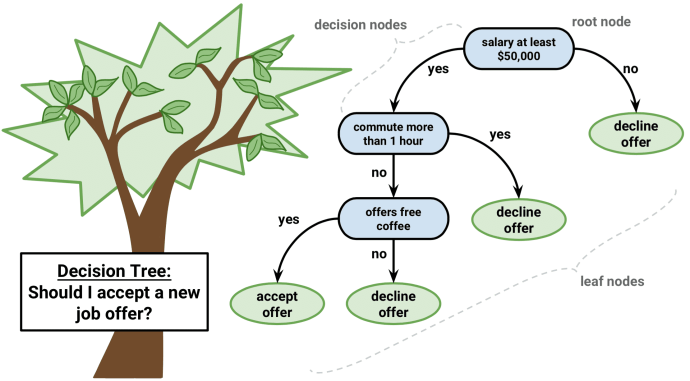
\includegraphics[height=5em]{images/decision_tree.png}} ;
\node (neural) at (4,2) {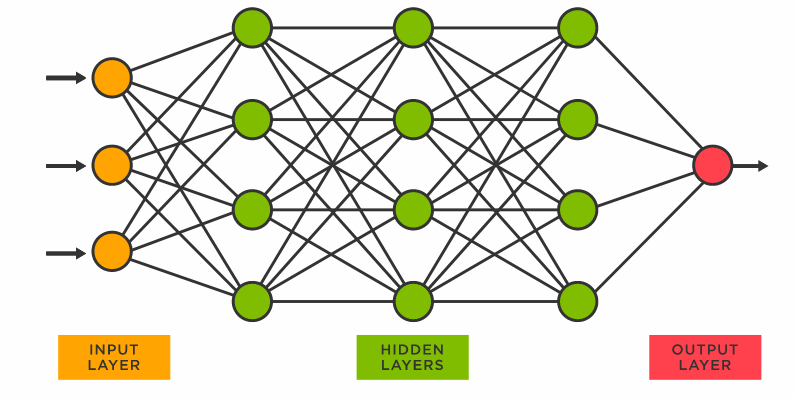
\includegraphics[height=5em]{images/neuralnetwork.png}} ;

\end{tikzpicture}
\end{center}

\end{frame}
\end{withoutheadline}

%---------------------------------------------------------------------------------------%

\begin{withoutheadline}
\begin{frame}[fragile]

\frametitle{Programmation logique inductive}

\begin{itemize}
 
\vfill
\pause
\item Connaissances de base

\begin{center}
\begin{minipage}{8.5cm}
\begin{block}{}
\begin{lstlisting}[basicstyle=\scriptsize]
parent(anne,marie).      femme(anne).
parent(anne,tom).        femme(marie).
parent(tom,eve).         femme(eve).
\end{lstlisting}
\end{block}
\end{minipage}
\end{center}

\vfill
\pause
\item Information positive et négative

\begin{center}
\begin{minipage}{8.5cm}
\begin{block}{}
\begin{lstlisting}[basicstyle=\scriptsize]
+ fille(marie,anne).    - fille(tom,anne).
+ fille(eve,tom).       - fille(tom,eve).
\end{lstlisting}
\end{block}
\end{minipage}
\end{center}

\vfill
\pause
\item Relation induite
\begin{center}
\begin{minipage}{8.5cm}
\begin{block}{}
\begin{lstlisting}[basicstyle=\scriptsize]
fille(X,Y) :- parent(Y,X), fille(X).
\end{lstlisting}
\end{block}
\end{minipage}
\end{center}

\vfill
\end{itemize}

\end{frame}
\end{withoutheadline}

%--------------------------------------------------------------------------%

\begin{withoutheadline}
\begin{frame}

\frametitle{Stratégie de base}

\vfill
\hspace*{-1.1cm}
\begin{tikzpicture}
\only<1->{
  \node (top) at (0,6) {\scriptsize \begin{tabular}{c}
                 fille(X,Y) :- vrai \\ \textit{\tiny (p=2, n=2, f=-1)}
                 \end{tabular}} ;
}

\only<2->{
  \node (p) at (-4,4) {\scriptsize \begin{tabular}{c}
      fille(X,Y) :- parent(Y,X). \\ \textit{\tiny (p=2, n=1, f=0)}
  \end{tabular}} ;
}

\only<4->{
  \node (e) at (0,4.5) {\scriptsize fille(X,Y) :- ...} ;
}

\only<3->{
  \node (f) at (4,4) {\scriptsize \begin{tabular}{c}
      fille(X,Y) :- femme(X). \\ \textit{\tiny (p=2, n=1, f=-1)}
  \end{tabular}} ;
}

\only<5->{
  \node (c) at (-4,1.5) {\scriptsize \begin{tabular}{c}
      fille(X,Y) :- parent(Y,X), femme(X). \\ \textit{\tiny (p=2, n=0, f=0)}
  \end{tabular}} ;
}

\only<6->{
  \node (w) at (2,2.5) {\scriptsize \begin{tabular}{c}
      fille(X,Y) :- parent(Y,X), femme(Y). \\ \textit{\tiny (p=2, n=1, f=-1)}
  \end{tabular} } ;
}

\only<2->{\draw[-latex] (top) -- (p); }
\only<4->{\draw[-latex] (top) -- (e);  }
\only<3->{\draw[-latex] (top) -- (f);  }
\only<5->{\draw[-latex] (p) -- (c);  }
\only<6->{\draw[-latex] (p) -- (w);  }

\end{tikzpicture}

\vfill
\only<7->{
\begin{center}
\begin{minipage}{6cm}
\begin{block}{\centering Caractéristiques}
\centering Incrémental \& à base de théorie
\end{block}
\end{minipage}
\end{center}
}

\vfill
\end{frame}
\end{withoutheadline}

%----------------------------------------------------------------------%

\begin{withoutheadline}
\begin{frame}

\frametitle{Contribution}

\vfill
\begin{alertblock}{Enjeu}
  Comprendre finement le processus d'apprentissage ainsi que des
  modèles produits
\end{alertblock}

\vfill
\begin{block}{Le notebook en deux mots}

  \begin{itemize}

  \item créer des contextes d'exécution personnalisés

  \item exécuter des requêtes Prolog permettant de
    \begin{itemize}
      \item tester le code introduit
      \item différentes hypothèses de travail
    \end{itemize}

  \item introduire des concepts auxiliaires de haut niveau
    
  \item générer des modèles par différentes méthodes

  \item inspecter les résultats intermédiaires 

  \end{itemize}
\end{block}


\vfill
\end{frame}
\end{withoutheadline}

\begin{withoutheadline}
\begin{frame}{Notebook Andante}
\hspace*{-.65cm}
\animategraphics[autoplay,loop,width=1.1\linewidth]{1.5}{images/andante/andante-}{0}{48}
\end{frame}
\end{withoutheadline}

%----------------------------------------------------------------------%
  

\end{document}

